%%%%%%%%%%%%%%%%%%%%%%%%%%%%%%%%%%%%%%%%%
% Beamer Presentation
% LaTeX Template
% Version 1.0 (10/11/12)
%
% This template has been downloaded from:
% http://www.LaTeXTemplates.com
%
% License:
% CC BY-NC-SA 3.0 (http://creativecommons.org/licenses/by-nc-sa/3.0/)
%
%%%%%%%%%%%%%%%%%%%%%%%%%%%%%%%%%%%%%%%%%

%----------------------------------------------------------------------------------------
%	PACKAGES AND THEMES
%----------------------------------------------------------------------------------------

\documentclass{beamer}

\mode<presentation> {

% The Beamer class comes with a number of default slide themes
% which change the colors and layouts of slides. Below this is a list
% of all the themes, uncomment each in turn to see what they look like.

%\usetheme{default}
%\usetheme{AnnArbor}
%\usetheme{Antibes}
%\usetheme{Bergen}
%\usetheme{Berkeley}
%\usetheme{Berlin}
%\usetheme{Boadilla}
%\usetheme{CambridgeUS}
%\usetheme{Copenhagen}
%\usetheme{Darmstadt}
%\usetheme{Dresden}
%\usetheme{Frankfurt}
%\usetheme{Goettingen}
%\usetheme{Hannover}
%\usetheme{Ilmenau}
%\usetheme{JuanLesPins}
%\usetheme{Luebeck}
\usetheme{Madrid}
%\usetheme{Malmoe}
%\usetheme{Marburg}
%\usetheme{Montpellier}
%\usetheme{PaloAlto}
%\usetheme{Pittsburgh}
%\usetheme{Rochester}
%\usetheme{Singapore}
%\usetheme{Szeged}
%\usetheme{Warsaw}

% As well as themes, the Beamer class has a number of color themes
% for any slide theme. Uncomment each of these in turn to see how it
% changes the colors of your current slide theme.

%\usecolortheme{albatross}
%\usecolortheme{beaver}
%\usecolortheme{beetle}
%\usecolortheme{crane}
%\usecolortheme{dolphin}
%\usecolortheme{dove}
%\usecolortheme{fly}
%\usecolortheme{lily}
%\usecolortheme{orchid}
%\usecolortheme{rose}
%\usecolortheme{seagull}
%\usecolortheme{seahorse}
%\usecolortheme{whale}
%\usecolortheme{wolverine}

%\setbeamertemplate{footline} % To remove the footer line in all slides uncomment this line
%\setbeamertemplate{footline}[page number] % To replace the footer line in all slides with a simple slide count uncomment this line

%\setbeamertemplate{navigation symbols}{} % To remove the navigation symbols from the bottom of all slides uncomment this line
}

\usepackage{graphicx} % Allows including images
\usepackage{booktabs} % Allows the use of \toprule, \midrule and \bottomrule in tables

\usepackage{polyglossia}
\setdefaultlanguage{german}

\definecolor{beamer@tu}{rgb}{0.5176,0.7215,0.0980} % changed this
%\setbeamercolor{alerted text}{fg=beamer@tu}
\setbeamercolor{structure}{fg=beamer@tu}

\setbeamertemplate{navigation symbols}{}

\usepackage[
locale=DE,
separate-uncertainty=true,
per-mode=symbol-or-fraction,
]{siunitx}
\sisetup{math-micro=\text{µ},text-micro=µ}
\usepackage{isotope}

%----------------------------------------------------------------------------------------
%	TITLE PAGE
%----------------------------------------------------------------------------------------

\title[Proseminar CI in Spielen]{Darwin's Avatars} % The short title appears at the bottom of every slide, the full title is only on the title page

\author{Christopher Riesner, Marian Kleineberg} % Your name
\institute[] % Your institution as it will appear on the bottom of every slide, may be shorthand to save space
{
Technische Universität Dortmund \\ % Your institution for the title page
\medskip
christopher.riesner@tu-dortmund.de\\ marian.kleineberg@tu-dortmund.de % Your email address
}
\date{9. Dezember 2016} % Date, can be changed to a custom date

\usepackage{multicol}



\begin{document}

\begin{frame}[noframenumbering]
\titlepage % Print the title page as the first slide
\end{frame}

%\begin{frame}
%\frametitle{Übersicht}
%\tableofconten
%\end{frame}

%----------------------------------------------------------------------------------------
%	PRESENTATION SLIDES
%----------------------------------------------------------------------------------------

\begin{frame}
	\frametitle{Teil 1}
	\textbf{Beginn der Präsentation}\\
\end{frame}

\usebackgroundtemplate{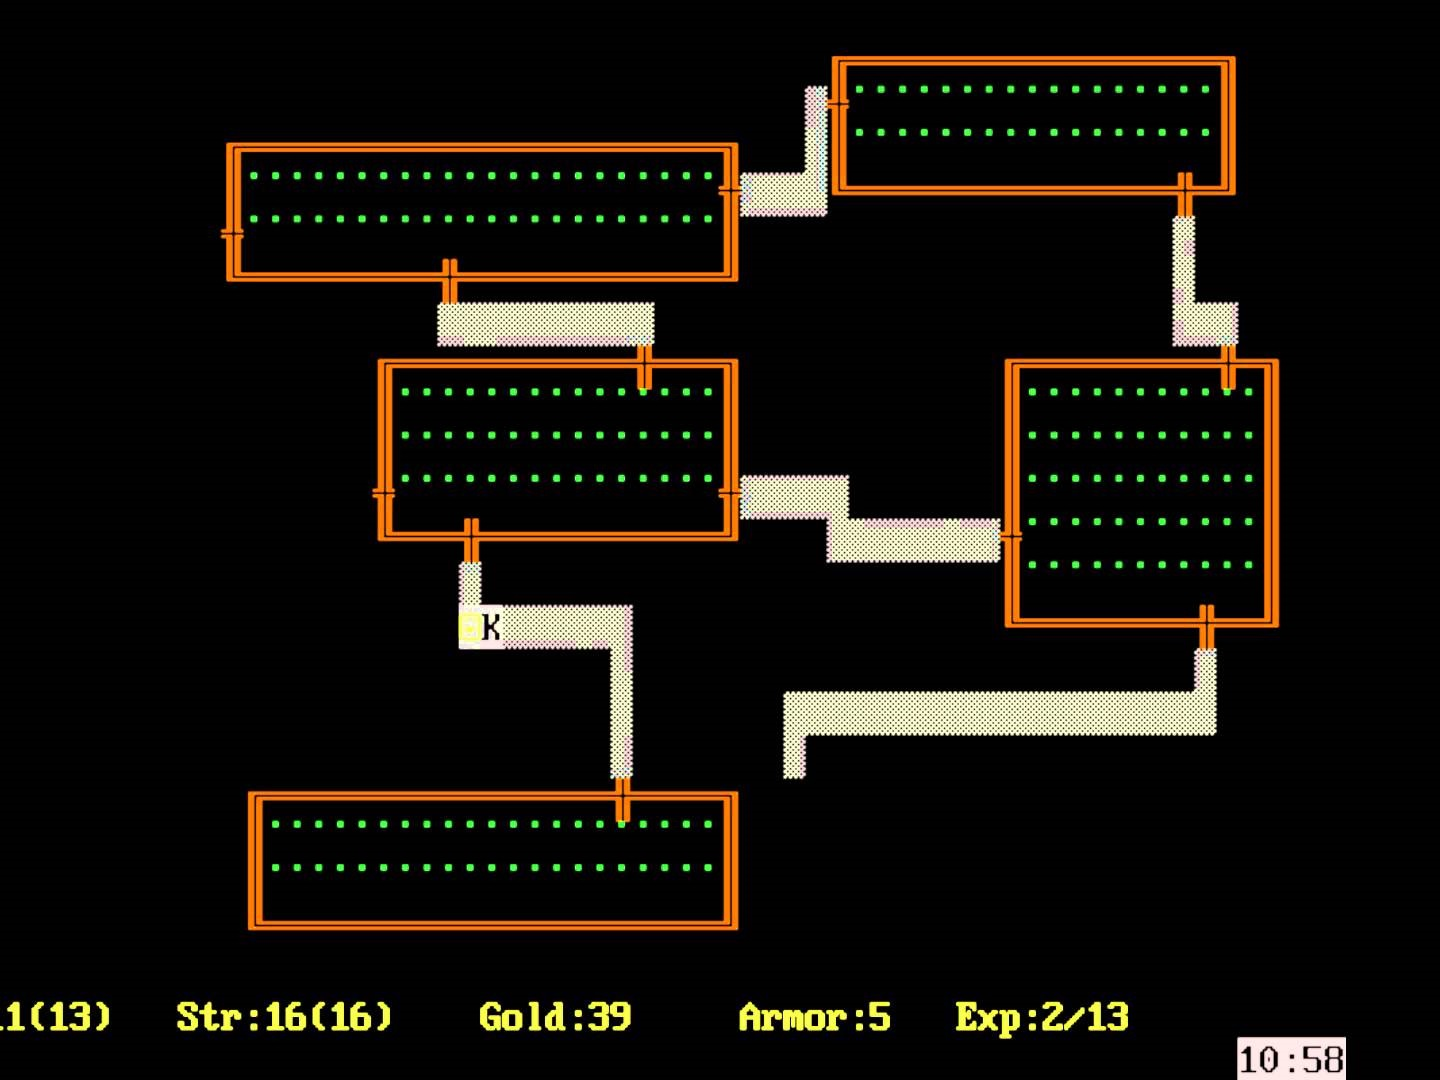
\includegraphics[width=\paperwidth]{games/rogue.jpg}}
\begin{frame}[plain]
\end{frame}

\usebackgroundtemplate{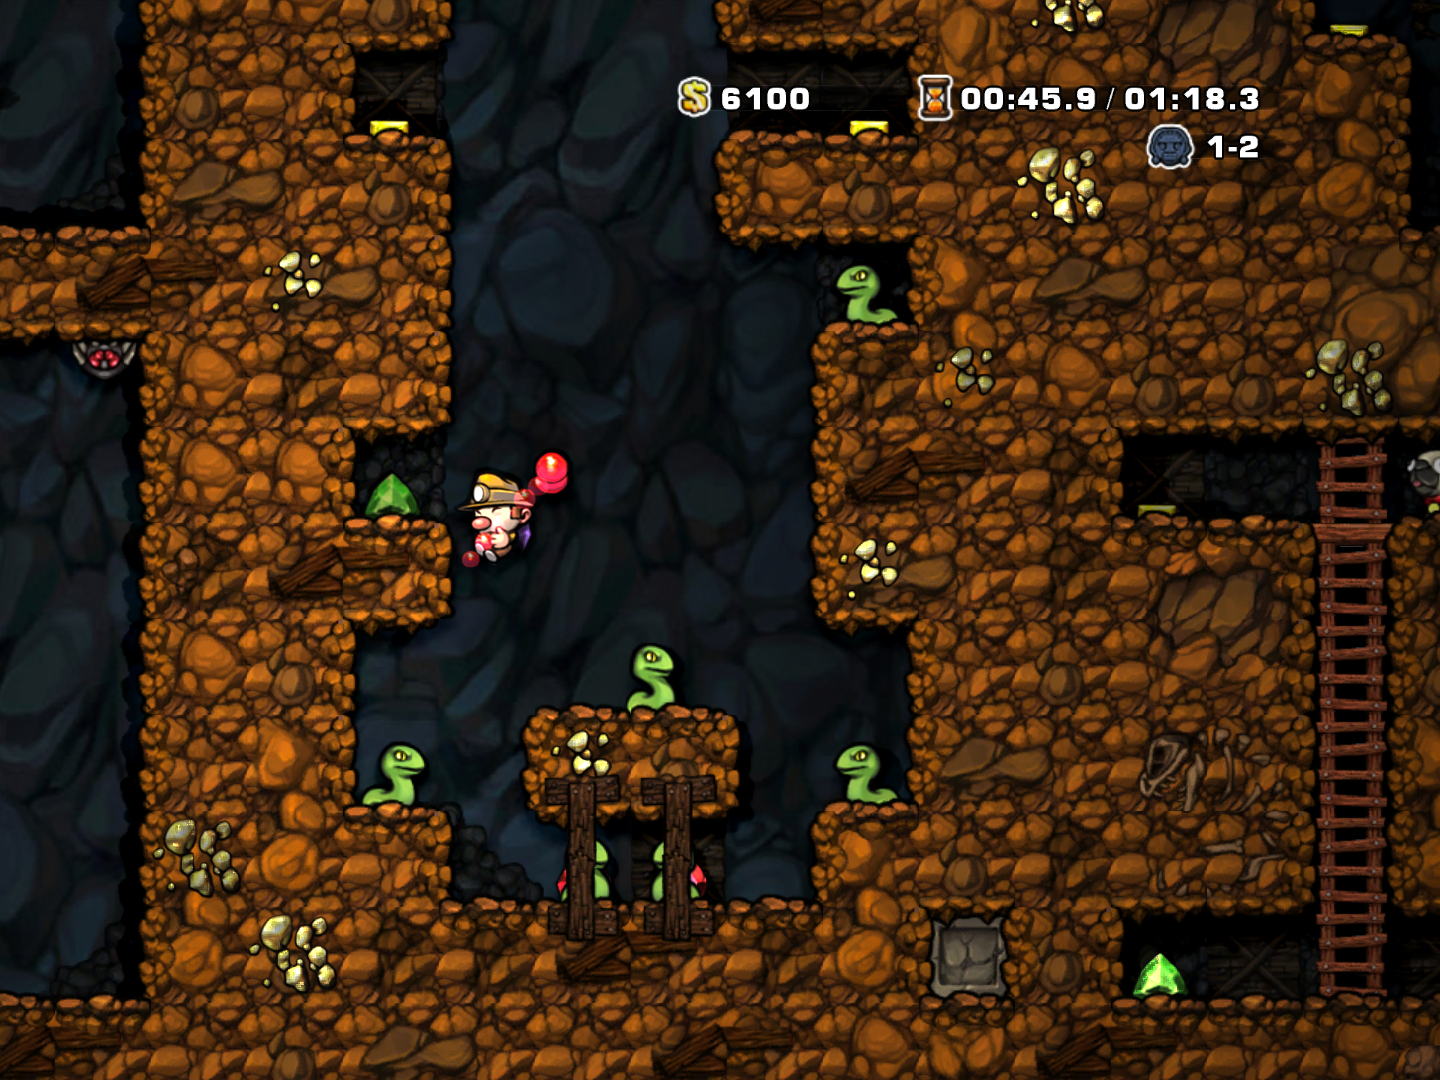
\includegraphics[width=\paperwidth]{games/spelunky.png}}
\begin{frame}[plain]
\end{frame}

\usebackgroundtemplate{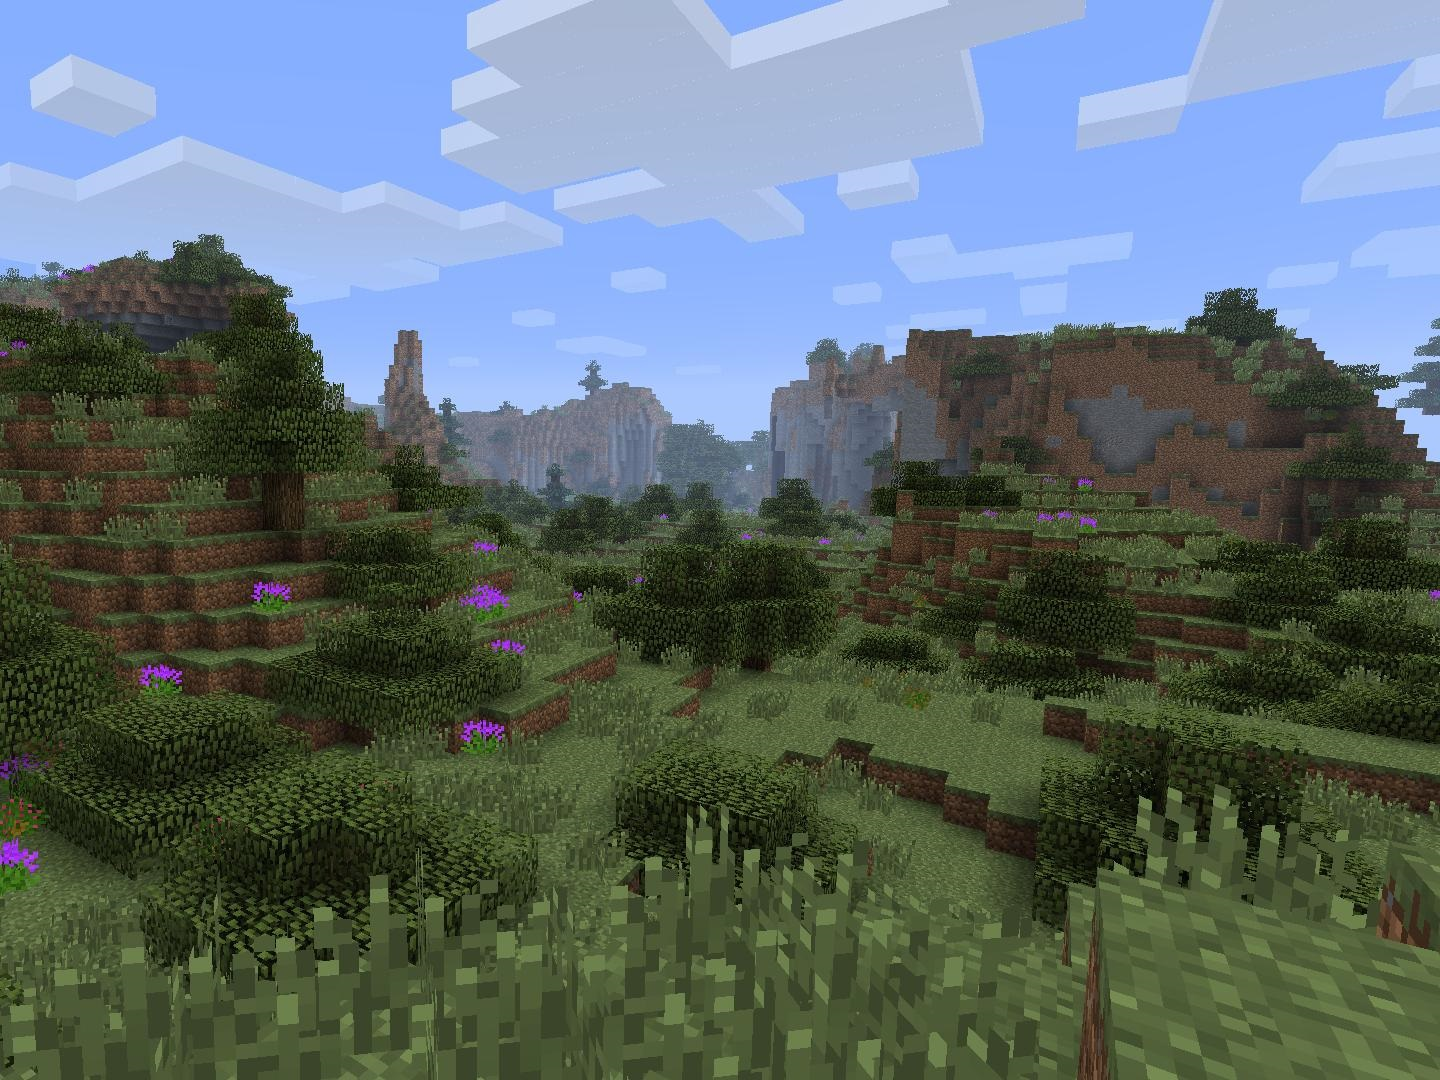
\includegraphics[width=\paperwidth]{games/minecraft.jpg}}
\begin{frame}[plain]
\end{frame}

\usebackgroundtemplate{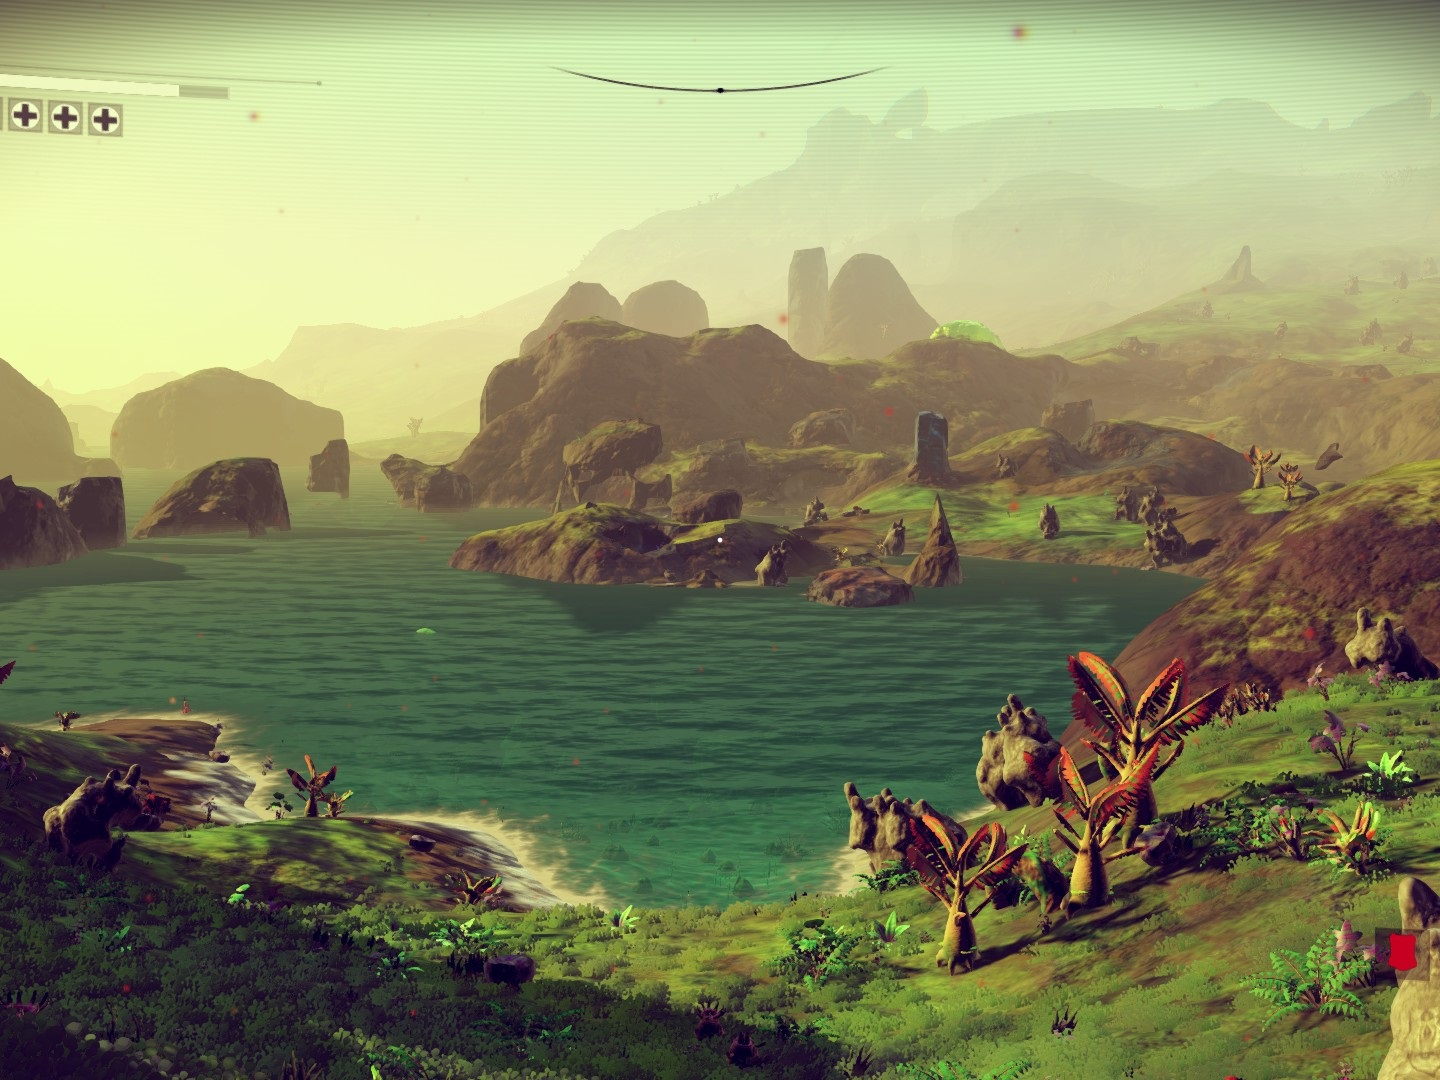
\includegraphics[width=\paperwidth]{games/nms1.jpg}}
\begin{frame}[plain]
\end{frame}

\usebackgroundtemplate{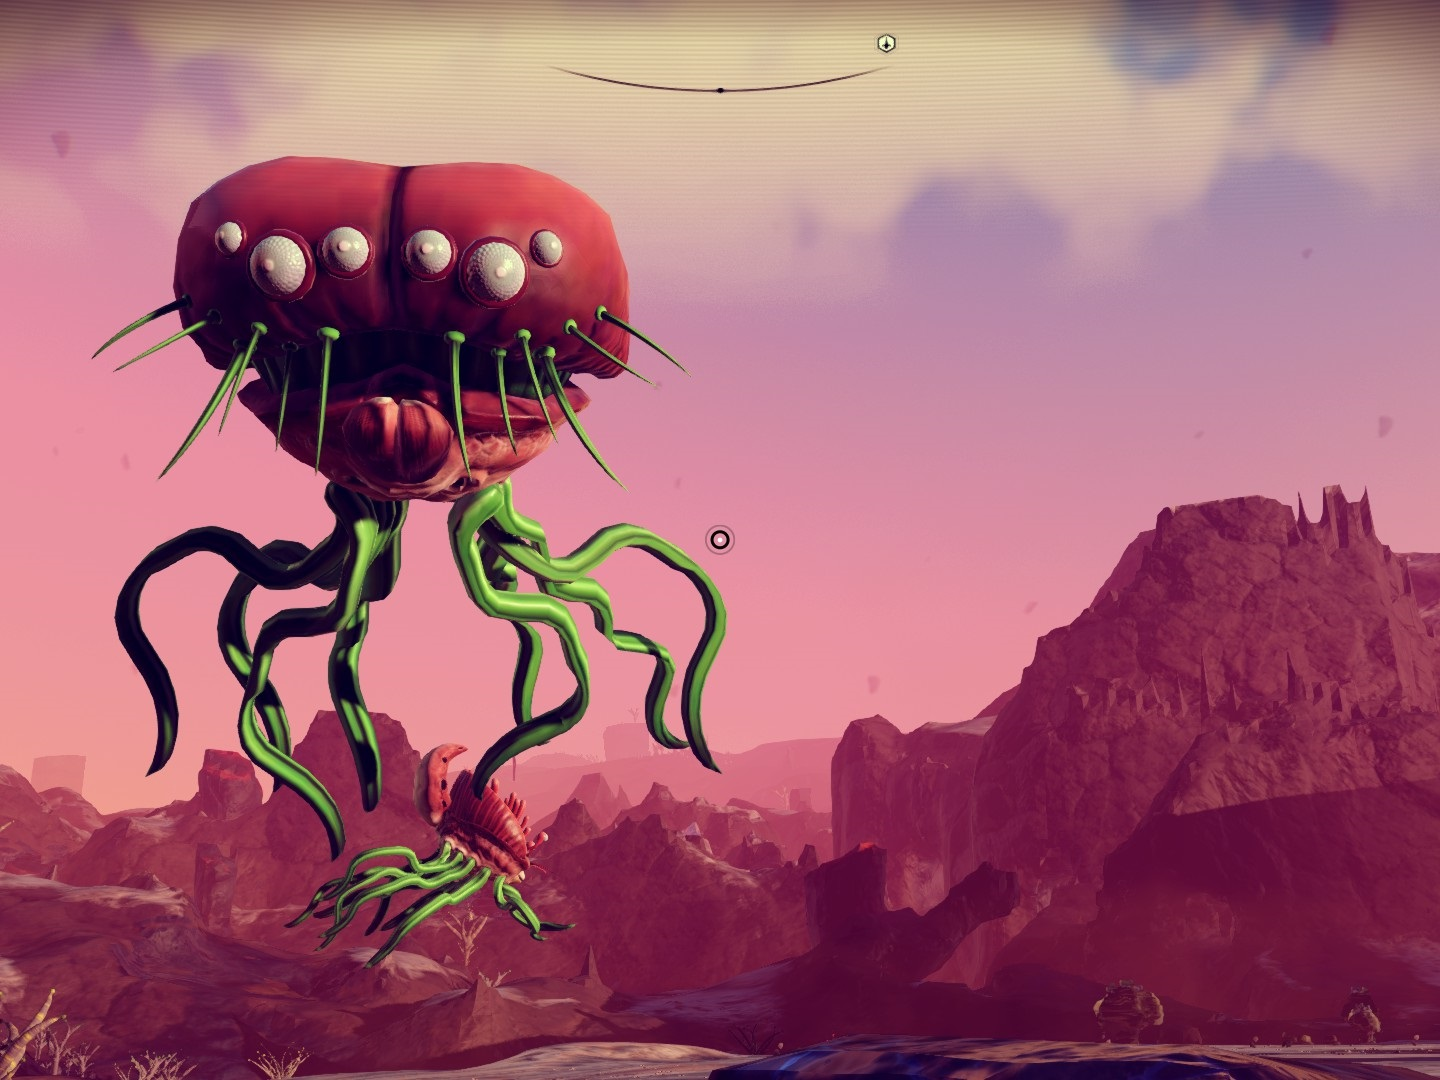
\includegraphics[width=\paperwidth]{games/nms2.jpg}}
\begin{frame}[plain]
\end{frame}

\usebackgroundtemplate{}

\begin{frame}
	\frametitle{Spiel}
	\textbf{Darwin's Avatars}\\
	\vspace{0.5em}
	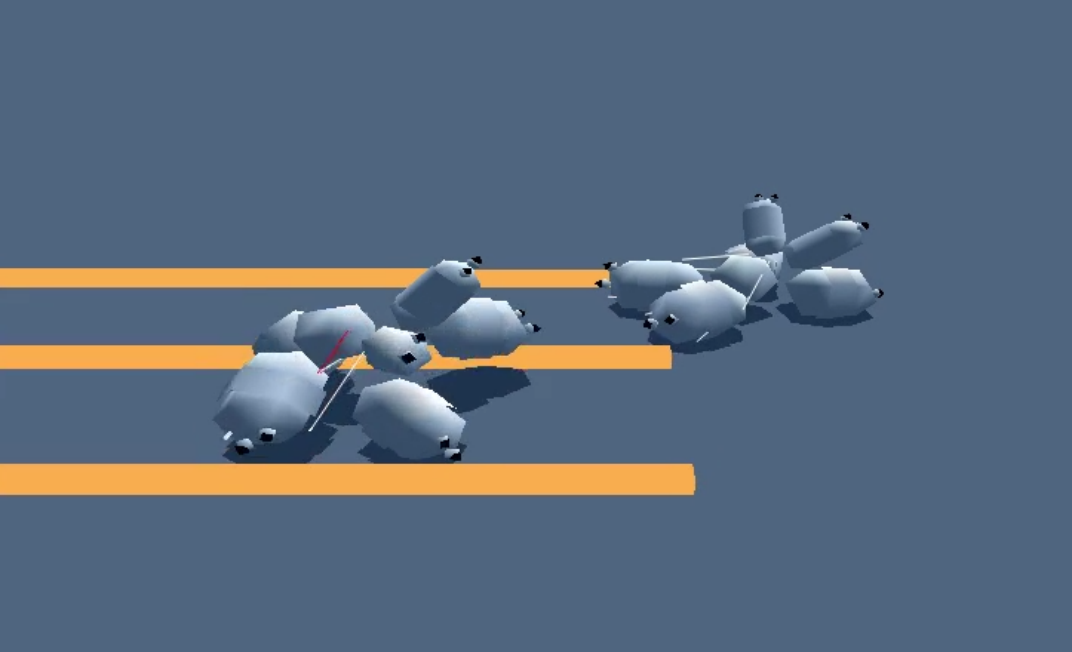
\includegraphics[width=\textwidth]{games/darwin.png}
\end{frame}

\begin{frame}
	\frametitle{Darwin's Avatars}
	\textbf{Vorgehensweise}\\ \pause
	\begin{itemize}
		\item Entwickle Körper und Gehirn evolutionär \pause
		\begin{itemize}
			\item Fitness = Spielziel \pause
		\end{itemize} 
		\item Entferne Gehirn \pause
		\item Spieler steuert die Kreatur \pause
		\item Messe Zeit bzw. Geschwindigkeit
	\end{itemize}	
\end{frame}

\begin{frame}
	\frametitle{Teil 2}
	\textbf{Visualisierung eines Sachverhalts}\\
\end{frame}

\begin{frame}
	\frametitle{Kodierung von Evolved Virtual Creatures (EVCs)}
	\begin{columns}[c]
		\column{.4\textwidth}
		\centering
		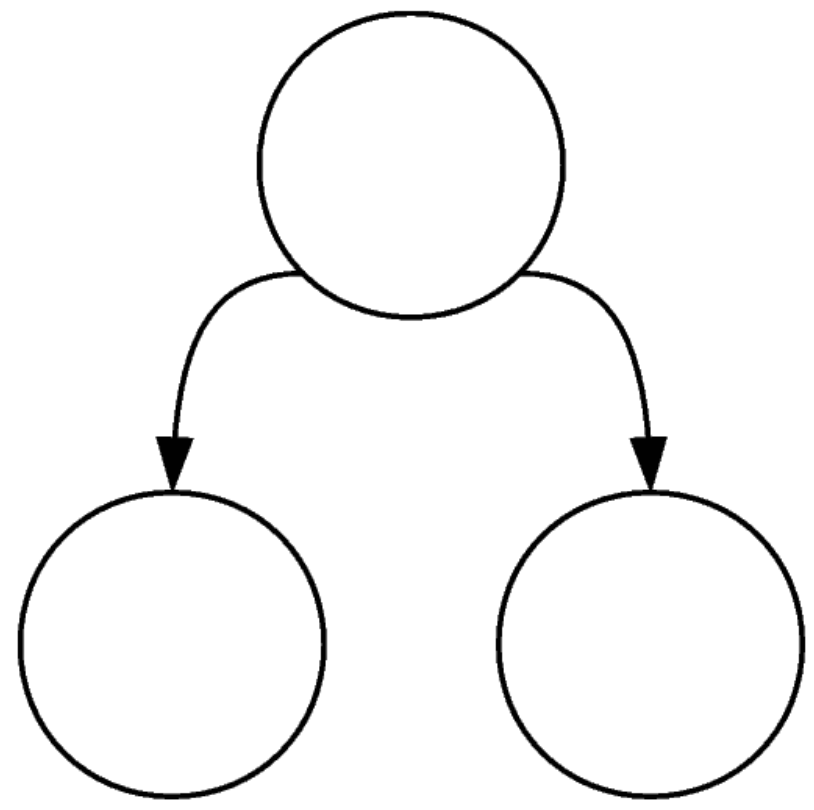
\includegraphics[width=0.7\textwidth]{g1.png} \pause
		\column{.6\textwidth}
		\centering
		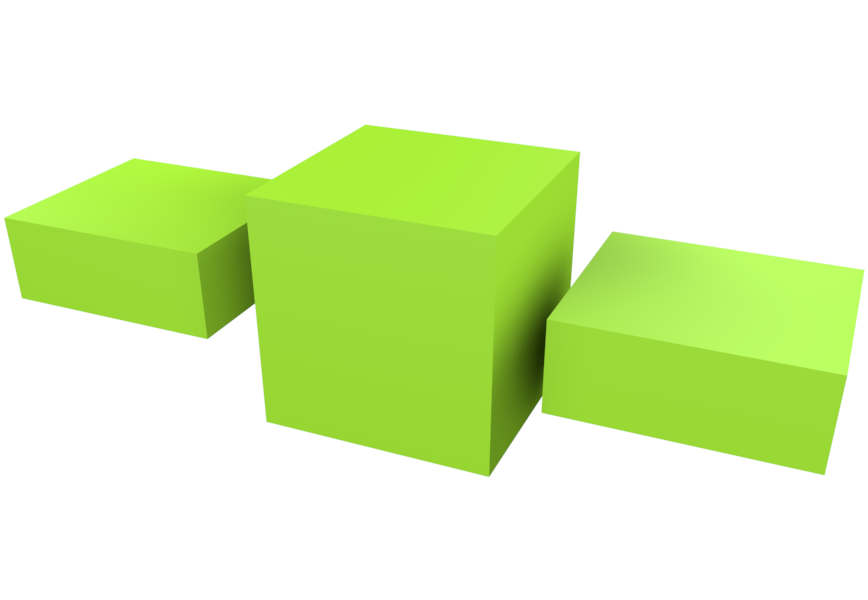
\includegraphics[width=\textwidth]{1.png}
	\end{columns}
\end{frame}

\begin{frame}
	\frametitle{Kodierung von Evolved Virtual Creatures (EVCs)}
	\begin{columns}[c]
		\column{.4\textwidth}
		\centering
		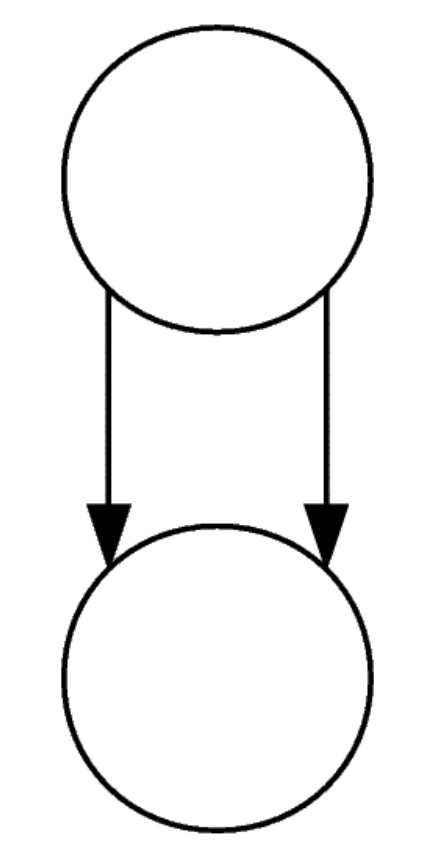
\includegraphics[width=0.4\textwidth]{g1a.png}
		\column{.6\textwidth}
		\centering
		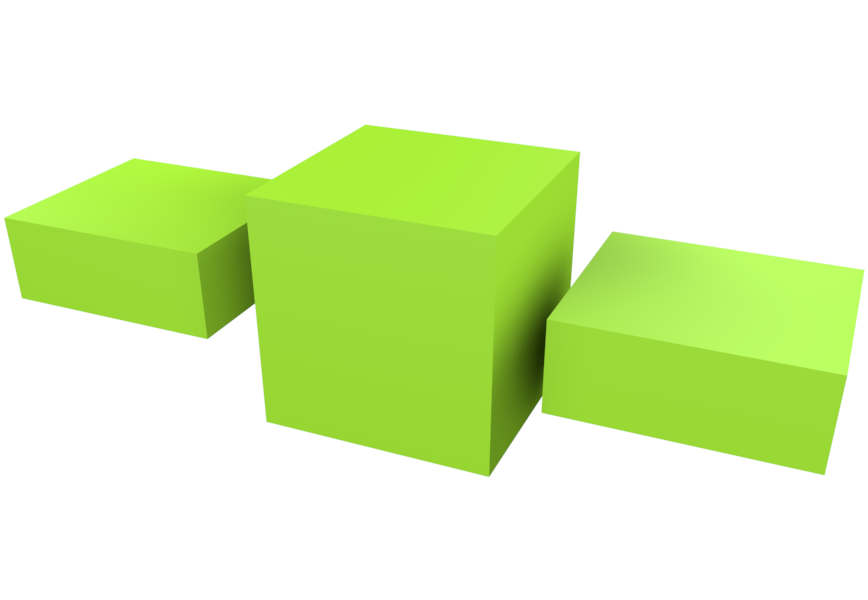
\includegraphics[width=\textwidth]{1.png}
	\end{columns}
\end{frame}

\begin{frame}
	\frametitle{Kodierung von Evolved Virtual Creatures (EVCs)}
	\begin{columns}[c]
		\column{.4\textwidth}
		\centering
		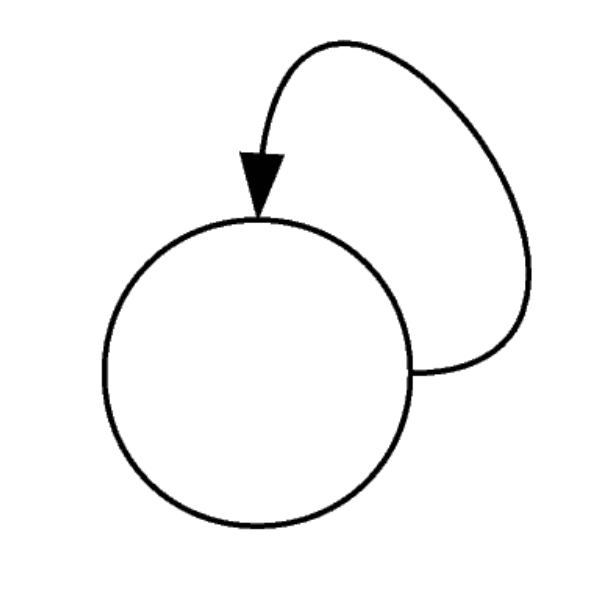
\includegraphics[width=0.7\textwidth]{g2.png} \pause
		\column{.6\textwidth}
		\centering
		
\includegraphics[width=0.8\textwidth]{2.png}
	\end{columns}
\end{frame}

\begin{frame}
	\frametitle{Kodierung von Evolved Virtual Creatures (EVCs)}
	\begin{columns}[c]
		\column{.4\textwidth}
		\centering
		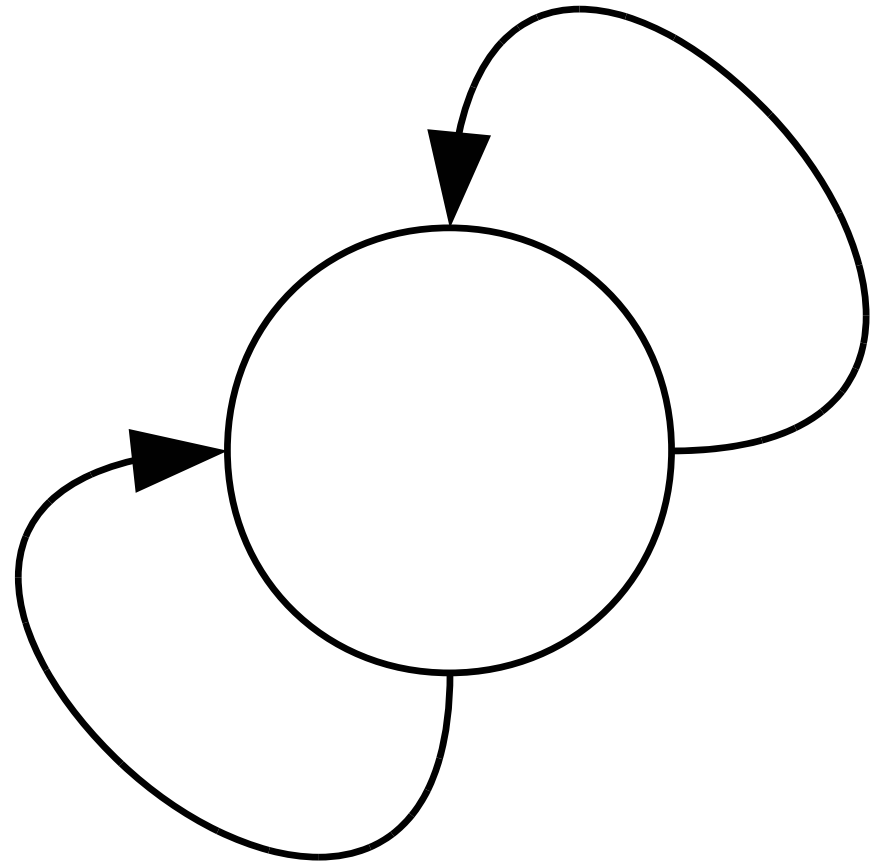
\includegraphics[width=0.7\textwidth]{g3.png} \pause
		\column{.6\textwidth}
		\centering
		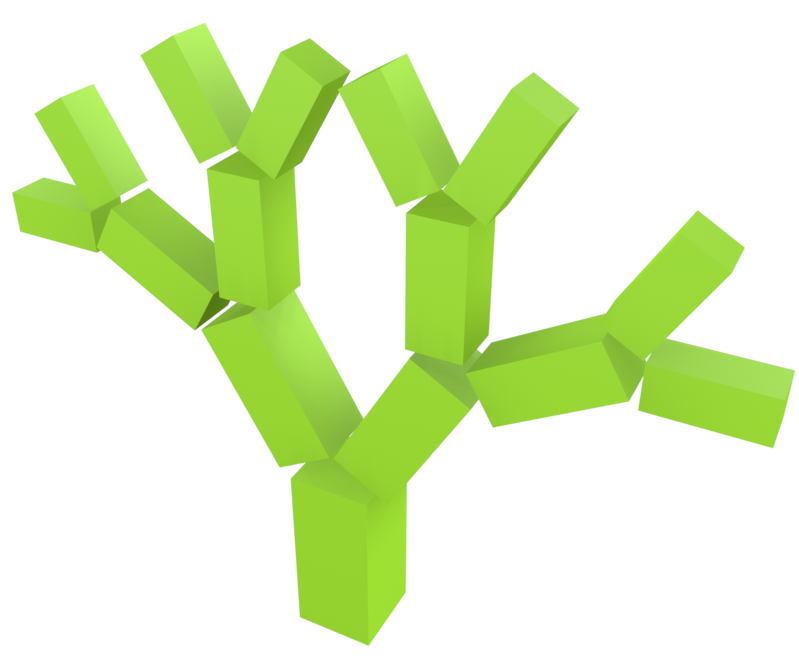
\includegraphics[width=\textwidth]{3.png}
	\end{columns}
\end{frame}

\begin{frame}
	\frametitle{Kodierung von Evolved Virtual Creatures (EVCs)}
	\begin{columns}[c]
		\column{.4\textwidth}
		\centering
		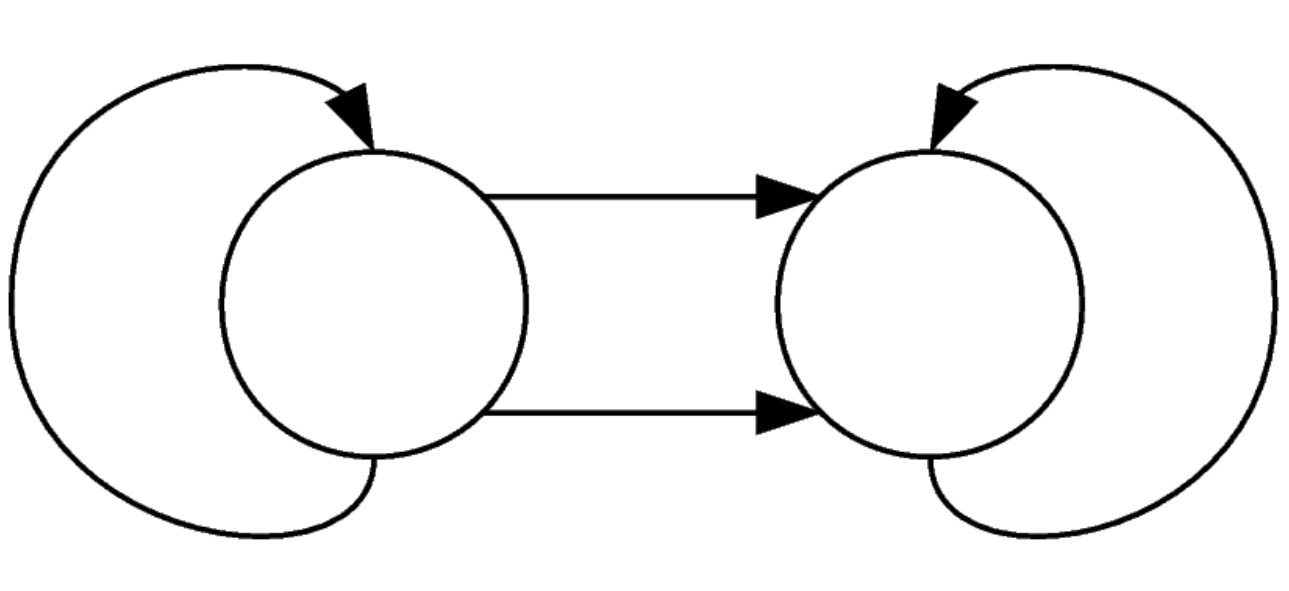
\includegraphics[width=0.9\textwidth]{g4.png} \pause
		\column{.6\textwidth}
		\centering
		
\includegraphics[width=\textwidth]{4.png}
	\end{columns}
\end{frame}


\begin{frame}
\frametitle{Teil 3}
\textbf{Kernbotschaft und Abschluss der Präsentation}\\
\end{frame}

\begin{frame}
	\frametitle{Zusammenfassung}
	\pause
	\textbf{Vorgehensweise}
	\begin{itemize}
		\item Körper und Gehirn werden gemeinsam entwickelt \pause
		\item Ersetze evolutionäres Gehirn durch menschlichen Spieler \pause
	\end{itemize}
	\vspace{1em}
	\textbf{Ergebnis}
	\begin{itemize}
		\item Tragfähiges Spielkonzept \pause
		\item Menschen sind evolutionärem Gehirn unterlegen \pause
	\end{itemize}
	\vspace{1em}
	\begin{block}{Take Home Message}
		Evolutionäre Kreaturen können verwendet werden, um interessante Spielgegenstände zu generieren, allerdings nicht in Echtzeit.	
	\end{block}
	
\end{frame}

\end{document} 